% Requires running Bibtex

\documentclass[%
reprint,
amsmath,amssymb,
aps,
floatfix
]{revtex4-2}

\usepackage{graphicx}% Include figure files
\usepackage{dcolumn}% Align table columns on decimal point
\usepackage{bm}% bold math
\usepackage{hyperref}% add hypertext capabilities
\usepackage[font=scriptsize,labelfont=bf, justification=justified]{caption}% change fontsize in captions
\usepackage{float}
\usepackage{booktabs}% cool table style
\hypersetup{
	colorlinks=true,       % false: boxed links; true: colored links
	linkcolor=black,        % color of internal links
	citecolor=black,        % color of links to bibliography
	filecolor=black,     % color of file links
	urlcolor=black         
}

\usepackage{listings}

%\usepackage{bibspacing}
%\setlength{\bibitemsep}{.5\baselineskip plus .05\baselineskip minus .05\baselineskip}


\begin{document}
	
	\preprint{APS/123-QED}
	
	\title{PHYC30170 Physics with Astronomy and Space Science Lab 1;\\Electronics}
	
	\author{Daragh Hollman}
	\email{daragh.hollman@ucdconnect.ie}
	
	\date{\today}
	
	\begin{abstract}
		
	\end{abstract}
	
	\maketitle
	
	\section{Introduction}
		Comment on the layout of the exercises and that some are being left out.
	
	\section{Exercise 5: RC Circuits}
		\subsection{Theory}
		What is an RC circuit? What is the expected outcome.\\
		
		Exercise 5 involves the construction and measurement of a RC circuit. An RC circuit is one which consists of a resistor and capacitor. The capacitor stores charge and the resistor controls the rate at which it discharges \cite{pumplin}. This time dependent discharge is an exponential decay given by the following equation:
		\begin{equation}
			V_\text{out} = V_\text{in} \exp{\left(\frac{-t}{RC}\right)}
			\label{eq:expDecay}
		\end{equation}where $V_\text{in}$ is the input voltage and $V_\text{out}$ is the voltage output measured by the voltmeter in figure \ref{fig:sampleRC}. $R$ and $C$ are simply the resistance and capacitance respectively. The factor $1/RC$ is defined as the decay constant which solely determines the rate of decay \cite{manual}.
		
		\begin{figure}
			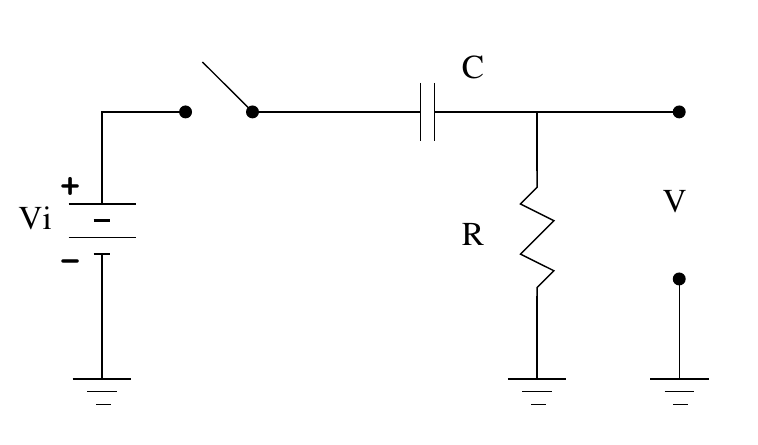
\includegraphics[width=0.85\columnwidth]{sampleRC.png}
			\caption{\label{fig:sampleRC}A sample RC circuit as described in the lab manual \cite{manual}.}
		\end{figure}
	
		\subsection{Methodology}
		The RC circuit depicted in figure \ref{fig:sampleRC} was constructed in DesignSoft's TINA \cite{TINA}, a circuit simulator. This construction is shown in figure \ref{fig:ex5Circuit}. A virtual oscilloscope was used in place of a voltmeter to measure the signal as a function of time. The component values of the capacitor and resistor were chosen as directed by the exercise and a square wave of frequency $20 \,\text{Hz}$ with peak to peak amplitude of $5\,\text{V}$ was used as the input. The circuit was simulated and the signal was recorded. The circuit was then constructed physically on a breadboard and the same measurement was made using an oscilloscope. The signals of the simulation, the measurement, and the analytical solution were then compared and the decay constants determined.
		
		\begin{figure}
			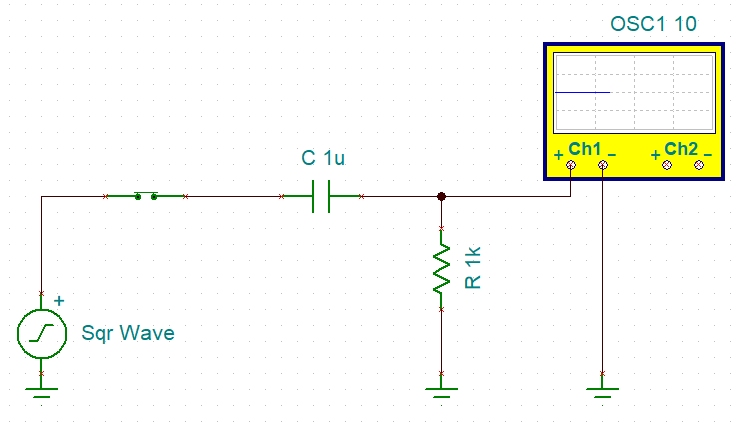
\includegraphics[width=0.85\columnwidth]{circuit_ex5.png}
			\caption{\label{fig:ex5Circuit}The circuit construction created in TINA for simulation.}
		\end{figure}
		
		\subsection{Results \& Analysis}
		The measured data from the breadboard were plotted in figure \ref{fig:ex5Results} along with the analytical solution calculated using equation \ref{eq:expDecay}. The decay constant of the analytical solution was calculated from the values of the resistor and the capacitor however, the decay constants for the measured data and simulation data were determined using least squares fitting of the signal. The decay constants for each method were recorded in table \ref{tab:decayConstants} along with their uncertainty which was determined by the square root of the diagonal elements of the covariance matrix. 
		
		\begin{table}[]
			\resizebox{0.85\columnwidth}{!}{%
				\begin{tabular}{@{}lll@{}}
					\toprule
					Method     & Decay Constant ($s^{-1}$) & Uncertainty \\ \midrule
					Analytical & 1000                    & N/A         \\
					Simulation & 1012.884                 & $\mathcal{O}10^{-6}$           \\
					Measured   & 895.937                  & $\mathcal{O}10^{-6}$           \\ \bottomrule
				\end{tabular}%
			}
			\caption{Decay constants for exercise 5. The uncertainties were determined by the square root of the diagonal elements of the covariance matrix for least squares fitting}
			\label{tab:decayConstants}
		\end{table}
		
	
		\begin{figure}
			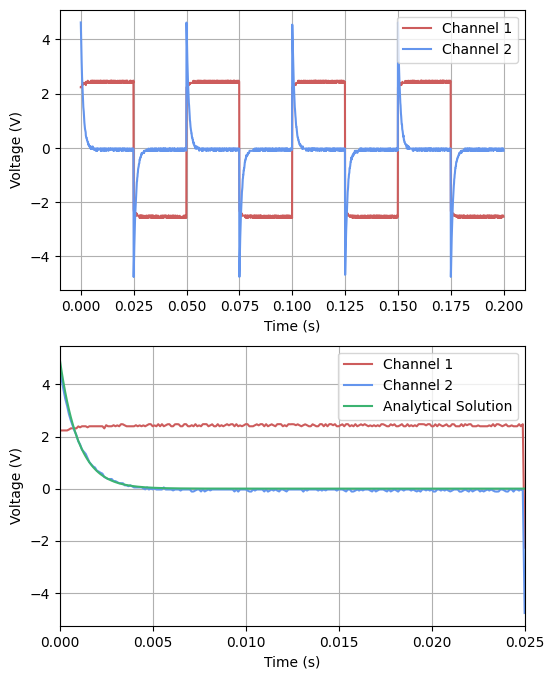
\includegraphics[width=0.85\columnwidth]{ex5_dualPlot.png}
			\caption{\label{fig:ex5Results}Input and output signals from the RC circuit in exercise 5. Channel 1 is the square wave driving the circuit whereas channel 2 is the output. The exponential decay response is clearly shown in the lower graph ($1\over2$ period) in comparison to the analytical solution.}
		\end{figure}
		\begin{figure}
			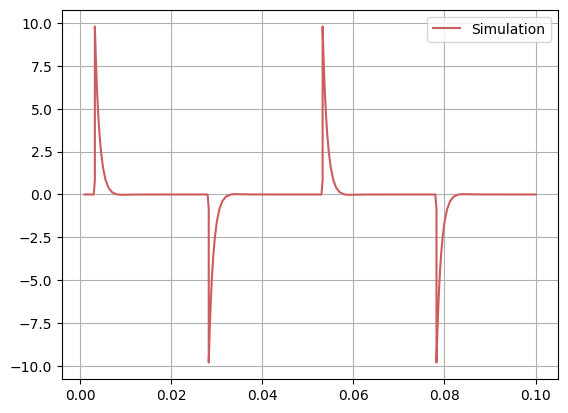
\includegraphics[width=0.85\columnwidth]{ex5_simPlot.png}
			\caption{\label{fig:ex5Sim}Simulation data generated by TINA, is exponential decay the same shape as the analytical and the measured.}
		\end{figure}
		\begin{figure}
			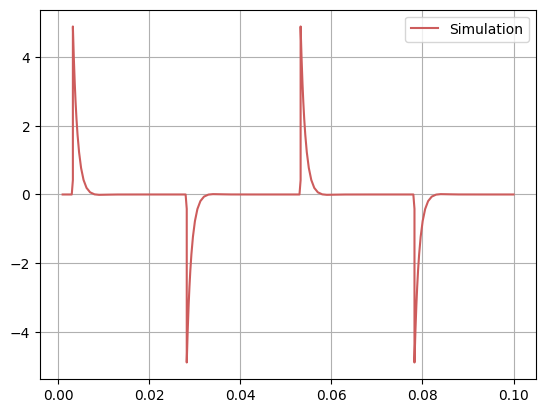
\includegraphics[width=0.85\columnwidth]{ex5_simPlotAdj.png}
			\caption{\label{fig:ex5SimAdj}The simulated data using peak to peak amplitude.}
		\end{figure}
	
		We notice that the amplitude of the simulation data is approximately twice that in the measured data. This is due to an inconsistency in the definition of amplitude, be it peak to peak amplitude or average to peak. We can still see clearly that the shape of the data matches what is expected and therefore dividing by two will yield the result under peak to peak amplitude. This is done explicitly in this exercise as shown in figures \ref{fig:ex5Sim} and \ref{fig:ex5SimAdj} however, for all further exercises where this applies - unless otherwise specified - this can be assumed to have been done.\\
		
		For consistency, in this report we shall use the term amplitude to refer to peak to peak amplitude as this is the definition used by the oscilloscope which was used to generate and measure signals for the majority of these exercises.
		
	\section{Exercise 7: RC Circuits and Frequency Filters}
		\subsection{Theory}
		Exercise 7 demonstrates how the same RC circuit as in exercise 5 can be used to make a high pass filter \cite{manual}. A high pass filter is a signal filter which allows higher frequencies to pass through unaffected but attenuates signals beyond a cut-off frequency. The combination of a resistor with a capacitor makes it possible to have voltage dividers dependent on frequency \cite{horowitz}. This frequency dependence arises from the impedance of the capacitor.
		\begin{equation}
			Z_C = -\frac{j}{\omega C}
		\end{equation}where $j$ is the imaginary number $j=\sqrt{-1}$, $C$ is the capacitance, and $\omega$ is the angular frequency. For the circuit in figure \ref{fig:sampleRC}, by Ohm's law we have a current:
		\begin{equation}
			I = \frac{V_\text{in}}{Z_\text{total}} = \frac{V_\text{in}}{R - Z_C}
		\end{equation}and hence we can calculate the voltage across the resistor, $V_\text{out}$, by substitution and rationalisation of the denominator:
		\begin{equation}
			V_\text{out} = I R = V_\text{in}\frac{[R+(\frac{j}{\omega C})]R}{R^2 + (\frac{1}{\omega^2 C^2})}
		\end{equation}with a magnitude of:
		\begin{equation}
			V_\text{out} = V_\text{in}\frac{R}{\left[R^2 + \left(\frac{1}{\omega^2 C^2}\right)\right]^\frac{1}{2}} = V_\text{in} \frac{\omega R C}{\left[1 + \left(\omega RC\right)^2\right]^\frac{1}{2}}
			\label{eq:amplitude}
		\end{equation}this is derived in full by Horowitz and Hill \cite{horowitz} where they also determine the phase analyticity to be:
		\begin{equation}
			\phi = \arctan\left(\frac{-1}{\omega RC}\right)
			\label{eq:phase}
		\end{equation}which derives from the total impedance.	
	
		\subsection{Methodology}
		The aim of this exercise was to simulate and measure the amplitude and phase response of the RC circuit from exercise 5 when driven by a sin wave. The circuit was designed and created in TINA as shown in figure \ref{fig:ex7Circuit}. Note that this circuit is predominantly the same as in figure \ref{fig:ex5Circuit} in exercise 5, with the only difference being in the wave generated by the voltage generator. The circuit was simulated and the amplitude and phase response were recorded. The circuit was then constructed physically and the amplitude and phase response were measured using an oscilloscope for frequencies of 1 Hz, 10 Hz, 100 Hz, 1 kHz, 10 kHz, 100 kHz, and 1 MHz.
		
		\begin{figure}
			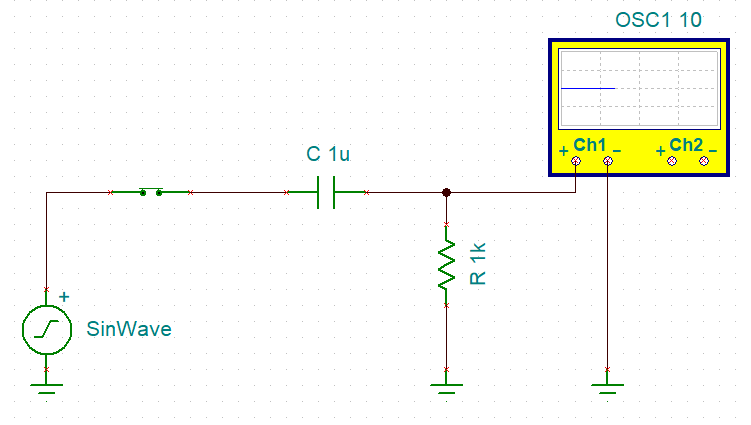
\includegraphics[width=0.85\columnwidth]{circuit_ex7.png}
			\caption{\label{fig:ex7Circuit}The circuit diagram created in TINA to measure the amplitude and phase response of an RC circuit.}
		\end{figure}
		\subsection{Results \& Analysis}
		The amplitude and phase data simulated by TINA was plotted in figure \ref{fig:ex7Results} along with the data measured from the physical circuit. It is clear that the data matches within the bounds of uncertainty. The uncertainty for these measurements were made either from the measuring limitations of the oscilloscope (i.e. the amount of decimals displayed) or where the measurement was not constant - such as in cases of low frequency ($<10 \,\text{Hz}$) - the average and standard deviation of 10 measurements was taken.\\
		
		These simulation curves displayed, and hence the data, match that described by equations \ref{eq:amplitude} and \ref{eq:phase}. We see that the circuit behaves at a high pass filter with negative gain for frequencies lower than $1 \,\text{kHz}$. The output is out of phase for these lower frequencies and results in destructive interference.
		
		\begin{figure}
			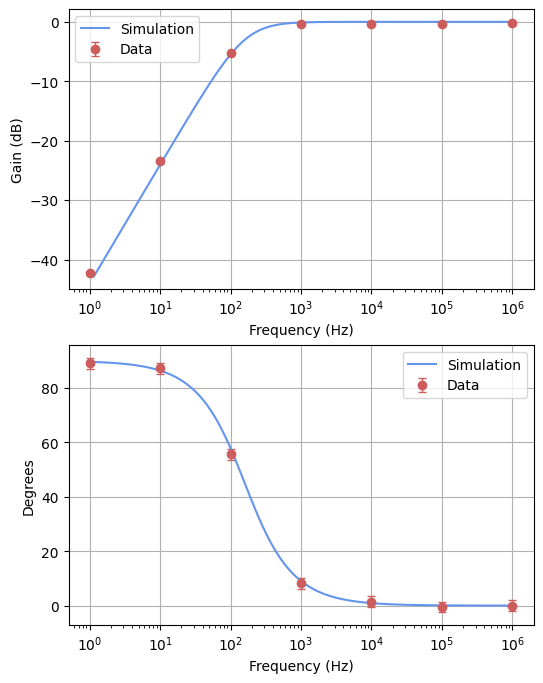
\includegraphics[width=0.85\columnwidth]{ex7_dualPlot.png}
			\caption{\label{fig:ex7Results}Bode plot of exercise 7. The circuit is a high pass filter with $R = 1 \text{k}\Omega$, $C = 1 \mu\text{F}$. Note that errorbars are included on both graphs however in some cases are to small to see.}
		\end{figure}
		
	\section{Exercise 12: }
		\subsection{Theory}
		The aim of exercise 12 is determine the I-V curve for a diode in forward and reverse bias. A diode is a PN junction which is either in forward bias or reverse bias depending on the direction of current flow across it \cite{manual}. 
		
		\subsection{Methodology}
		
		\begin{figure}
			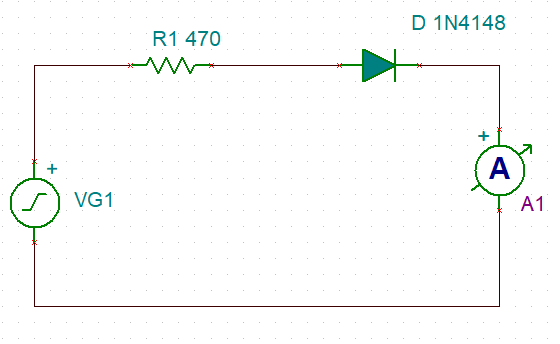
\includegraphics[width=0.85\columnwidth]{ex12Circuit.png}
			\caption{\label{fig:ex12Circuit}Circuit diagram create in TINA for exercise 12. Note that this doesn't include the capacitor added in the second half of the exercise.}
		\end{figure}
		\subsection{Results \& Analysis}
		
		...As the breakthrough voltage of the diode was much higher than the maximum output of the voltage generator and hence any leak-through voltage was too small to be measured by the voltmeter.
		\begin{figure}
			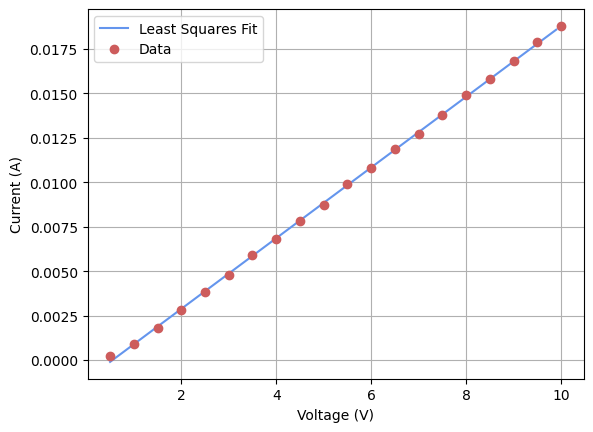
\includegraphics[width=0.85\columnwidth]{IVCurveLinear.png}
			\caption{\label{fig:IVCurveLinear}I-V curve for the circuit in forward bias. As the breakthrough voltage of the diode was much higher than the maximum output of the voltage generator and hence any leak-through voltage was too small to be measured by the voltmeter.}
		\end{figure}
		
	\section{Exercise 19: Transistors as a Current Amplifier}
		\subsection{Theory}
		A transistor is a 3 terminal semiconductor device comprised of the joining of two PN junctions. They can be arranged in two layouts, npn or pnp, see figure \ref{fig:transistors} \cite{horowitz}. In this exercise, a transistor is used as an amplifier. A small current $I_B$ must flow into the base to allow current $I_C$ to flow through the detector. The current gain - the ratio between these two currents - is determined by the following equation \cite{horowitz}.
		\begin{equation}
			\beta = {I_C \over I_B}
			\label{eq:currentGain}
		\end{equation}
		
		\begin{figure}
			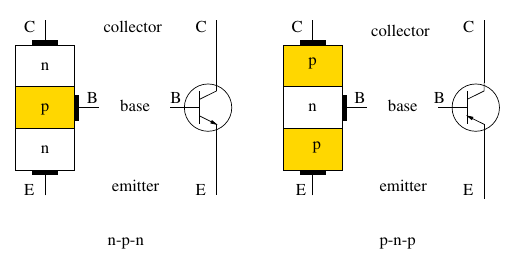
\includegraphics[width=0.85\columnwidth]{transistors.png}
			\caption{\label{fig:transistors}A diagram of the two layouts of transistors \cite{manual}.}
		\end{figure}
		
		\subsection{Methodology}
		
		This exercise aims to simulate a current amplifying circuit and calculate the current gain for a 2N4400 transistor. The circuit was designed and simulated in TINA, see figure \ref{fig:currentAmplifier}. The resistor values were chosen as given by the lab manual \cite{manual}, with their purpose being to reduce the current flow into the base of the transistor. The TINA software's DC analysis was used to measure the current from the ammeters. These currents were recorded and then equation \ref{eq:currentGain} was used to calculate the current gain based on the current running through the collector and the base.
		
		\begin{figure}
			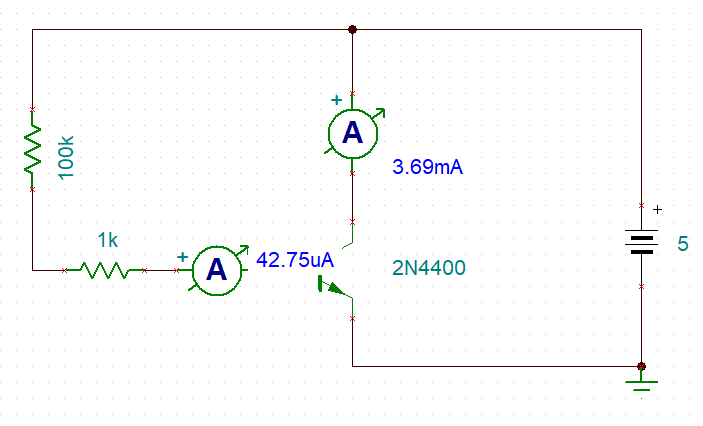
\includegraphics[width=0.85\columnwidth]{circuitOn.png}
			\caption{\label{fig:currentAmplifier}The circuit setup in TINA to demonstrate current amplification with transistors.}
		\end{figure}
		
		\subsection{Results \& Analysis}
		Equation \ref{eq:currentGain} was used to calculate the current gain of the circuit using the data from figure \ref{fig:currentAmplifier}. With a base current of $42.75 \,\mu\text{A}$ and a collector current of $3.69 \,\text{mA}$, the current gain, $\beta$, was calculated to be $\beta = 86.32$.
	
	\section{Exercise 20: Transistors as a Switch}
		\subsection{Theory}
		Another applications of transistors is as a switch. Make for good switches as they are small, cheap, reliable, and can switch rapidly \cite{manual}. Similarly to how the current amplifier required a current (and hence voltage) through the base to allow current to flow through the collector, if we think of the path from the collector to the emitter as the primary path, then the voltage at the base controls if the current can flow through this path. The "switch" is on if there is sufficient voltage at the base (approx. $0.7 \,\text{V}$), and off where there isn't.\\
		
		The aim this exercise is the vary the load resistance and look at the effect it has on the switching action. The load resistor is placed in series with the collector of the transistor. The output voltage from a sample circuit (figure \ref{fig:ex20Circuit}) is expected to look as shown in figure \ref{fig:loadResistorDiagram}. This graph is split up into three distinct sections. In section A the transistor switch is off, there is no current flowing from the collector and hence the output is 6 V. In section B, the transistor switch is partially on, as the current increases, the voltage across the load resistor increases and the output drops. In section C, the transistor is fully on and said to be saturated \cite{manual}.
		
		
		\begin{figure}
			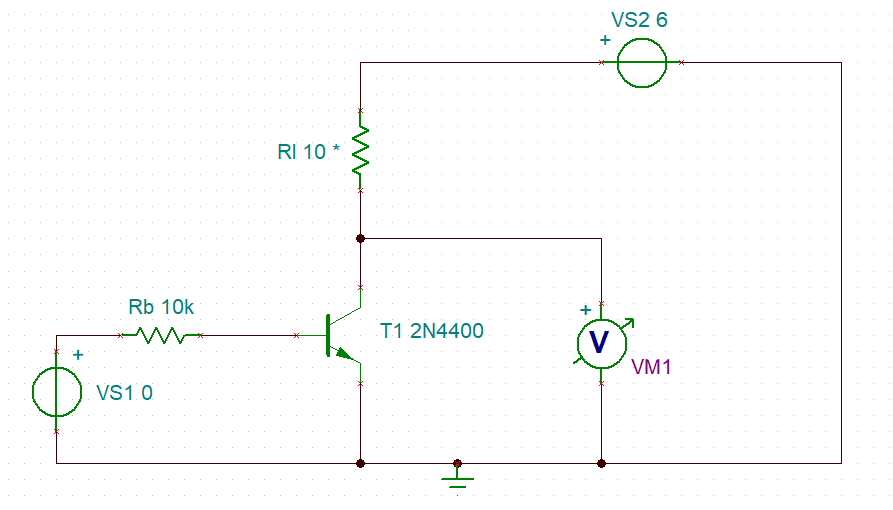
\includegraphics[width=0.85\columnwidth]{ex20Circuit.png}
			\caption{\label{fig:ex20Circuit}The circuit diagram for exercise 20, created in TINA. The load resistor, $Rl$, was setup so that it could be varied.}
		\end{figure}
		\begin{figure}
			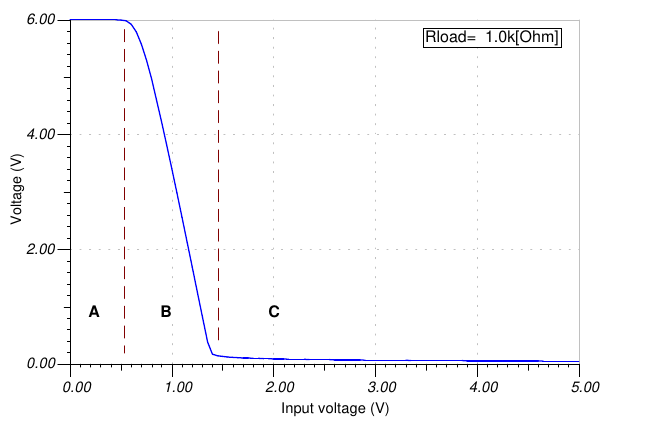
\includegraphics[width=0.85\columnwidth]{loadResistorDiagram.png}
			\caption{\label{fig:loadResistorDiagram}A diagram of the voltage response with a load resistor of resistance $1 \,\text{k}\Omega$ \cite{manual}.}
		\end{figure}
		
		
		\subsection{Methodology}
		
		The circuit was constructed in TINA as directed by the exercise \cite{manual}, see figure \ref{fig:ex20Circuit}. The load resistor was set up as a control target in TINA to vary its resistance during analysis. The voltage response for load resistances of $10\,\Omega$, $100\,\Omega$, $1\,\text{k}\Omega$, and $10\,\text{k}\Omega$ were simulated and recorded in figure \ref{fig:ex20Results}.
		
		\subsection{Results \& Analysis}
		
		Each voltage response simulation for each load resistor was recorded and plotted in figure \ref{fig:ex20Results}. We see that the results match that of what is expected in figure \ref{fig:loadResistorDiagram}. We see that the slope of the B section of the voltage response depends on the load resistance with a higher resistance yielding a sharper slope. The lower load resistances of $10\,\Omega$ and $100\,\Omega$ never reach saturation for an input voltage less than the voltage before the load resistor.
		
		\begin{figure}
			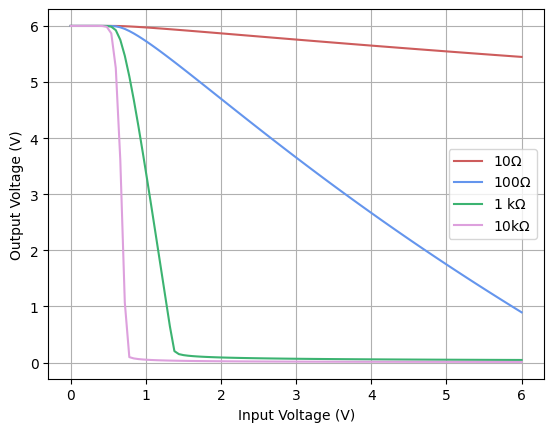
\includegraphics[width=0.85\columnwidth]{ex20Results}
			\caption{\label{fig:ex20Results}}
		\end{figure}
		
	\section{Exercise 21: LDR controlled switch}
		\subsection{Theory}
		In this exercise, an LDR is used in a voltage divider to control the voltage at the base of the transistor.
		
		\subsection{Methodology}
		The circuit was first designed in TINA as shown in figure \ref{ex21}
		
		\subsection{Results \& Analysis}
		
	\section{Exercise 25: }
		\subsection{Theory}
		\subsection{Methodology}
		\subsection{Results \& Analysis}
		
	\section{Exercise 27: }
		\subsection{Theory}
		\subsection{Methodology}
		\subsection{Results \& Analysis}
		
	\clearpage
	\bibliography{electronics.bib}% Produces the bibliography via BibTeX.
	
	\clearpage
	\onecolumngrid
	\appendix

	
	
\end{document}

